\documentclass[tikz,border=0pt]{standalone}
\usepackage{fontspec}
\usepackage{amsmath}
\usepackage{xcolor}
\usepackage{tikz}
\usepackage{pgfplots}
\pgfplotsset{compat=1.18}
\usetikzlibrary{arrows.meta,calc,fit,positioning,shapes.geometric,shapes.misc,patterns,plotmarks}
\IfFontExistsTF{Arial}{\setsansfont{Arial}}{\setsansfont{TeX Gyre Heros}}
\renewcommand{\familydefault}{\sfdefault}
\tikzset{
  >={Stealth[length=2.2mm,width=1.5mm]},
  exact title/.style={font=\bfseries\fontsize{10.5}{12}\selectfont,align=center},
  exact subtitle/.style={font=\fontsize{6.3}{7.2}\selectfont,align=center},
  exact label/.style={font=\fontsize{6.4}{7.5}\selectfont,align=center},
  exact tiny/.style={font=\fontsize{5.3}{6.3}\selectfont,align=center},
  panel/.style={draw=black!14,rounded corners=1.2mm,fill=white,line width=.45pt},
  neutral/.style={draw=black!30,fill=black!3,rounded corners=1mm,line width=.45pt},
  arrow/.style={-Stealth,line width=.7pt},
  softarrow/.style={-Stealth,line width=.55pt,draw=black!45},
  dashedarrow/.style={-Stealth,dashed,line width=.55pt,draw=black!55},
  metric/.style={font=\fontsize{5.3}{6.3}\selectfont,fill=white,inner sep=1pt},
}
\newcommand{\pill}[4]{\node[draw=#2!70,fill=#2!10,rounded corners=1.5mm,inner xsep=3pt,inner ysep=2pt,exact label,text=#2] (#1) at #3 {#4};}
\newcommand{\frameboxx}[4]{\draw[draw=#2!65,fill=#2!8,rounded corners=.6mm,line width=.5pt] (#1.south west) rectangle (#1.north east);\node[exact tiny,text=#2] at #3 {#4};}
\newcommand{\axislabel}[3]{\node[exact tiny,text=black!60] at (#1) {#2};\node[exact tiny,text=black!60,rotate=90] at (#3) {#2};}

\definecolor{nwmink}{HTML}{222222}
\definecolor{nwmact}{HTML}{F2D21B}
\definecolor{nwmgood}{HTML}{63B34A}
\definecolor{nwmbad}{HTML}{E4514E}
\begin{document}
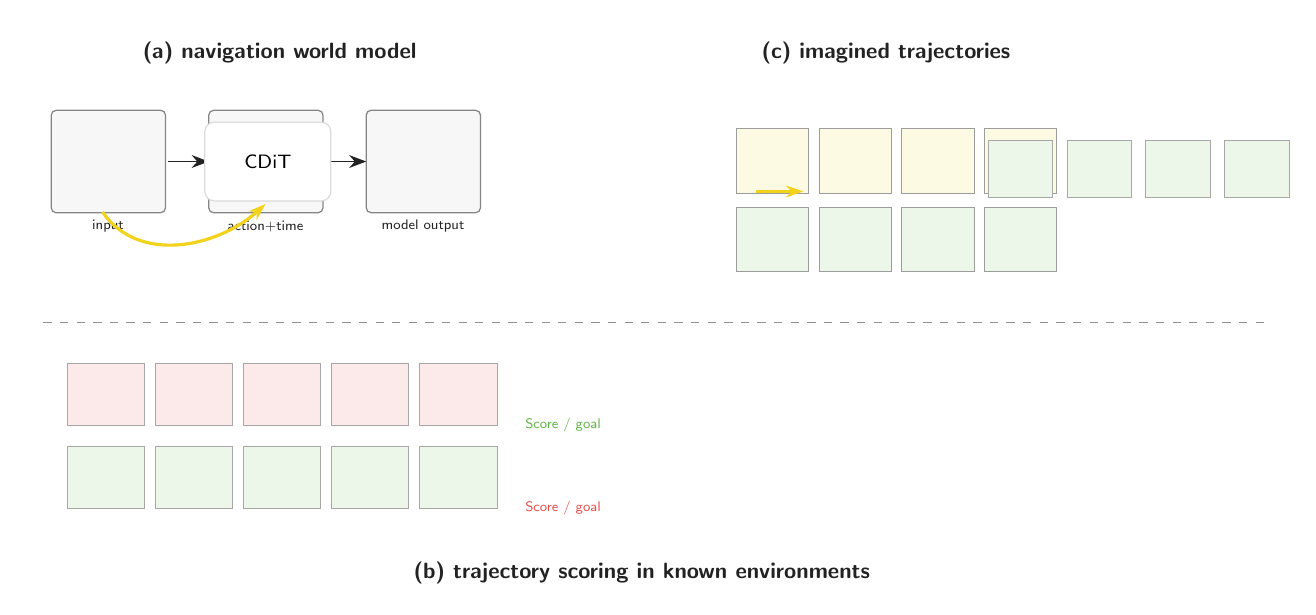
\begin{tikzpicture}[x=1cm,y=1cm]
\path[use as bounding box] (0,0) rectangle (16,7.1);
\node[font=\bfseries\fontsize{8.5}{9}\selectfont,text=nwmink] at (3.2,6.78) {(a) navigation world model};
\node[font=\bfseries\fontsize{8.5}{9}\selectfont,text=nwmink] at (10.9,6.78) {(c) imagined trajectories};
\node[font=\bfseries\fontsize{8.5}{9}\selectfont,text=nwmink] at (7.8,0.18) {(b) trajectory scoring in known environments};
\foreach \x/\lab in {0.3/input,2.3/action+time,4.3/model output}{
  \draw[draw=nwmink!55,fill=black!3,rounded corners=.6mm,line width=.45pt] (\x,4.75) rectangle +(1.45,1.3);
  \node[exact tiny,text=nwmink] at (\x+.72,4.58) {\lab};
}
\draw[arrow,draw=nwmink] (1.78,5.4)--(2.3,5.4);
\draw[arrow,draw=nwmink] (3.78,5.4)--(4.3,5.4);
\node[panel,minimum width=1.6cm,minimum height=1.0cm] at (3.05,5.4) {\scriptsize CDiT};
\draw[nwmact,line width=1.15pt,->] (0.95,4.76) .. controls (1.4,4.1) and (2.4,4.3) .. (3.02,4.86);
\foreach \c in {0,1,2,3}{
  \draw[draw=nwmink!45,fill=nwmact!12,line width=.3pt] (9.0+\c*1.05,5.0) rectangle +(0.92,.82);
  \draw[draw=nwmink!45,fill=nwmgood!12,line width=.3pt] (9.0+\c*1.05,4.0) rectangle +(0.92,.82);
}
\draw[nwmact,line width=1pt,->] (9.25,5.02)--(9.85,5.02);
\draw[dashed,draw=nwmink!50] (0.2,3.35)--(15.7,3.35);
\foreach \r/\col in {0/nwmgood,1/nwmbad}{\foreach \c in {0,1,2,3,4}{
  \draw[draw=nwmink!40,fill=\col!12,line width=.3pt] (0.5+\c*1.12,1.0+\r*1.05) rectangle +(0.98,.78);
}}
\node[exact tiny,text=nwmgood] at (6.8,2.05) {Score / goal};
\node[exact tiny,text=nwmbad] at (6.8,1.0) {Score / goal};
\foreach \x in {12.2,13.2,14.2,15.2}{\draw[draw=nwmink!40,fill=nwmgood!12,line width=.3pt] (\x,4.95) rectangle +(0.82,.72);}
\end{tikzpicture}
\end{document}
